% Options for packages loaded elsewhere
\PassOptionsToPackage{unicode}{hyperref}
\PassOptionsToPackage{hyphens}{url}
%
\documentclass[
]{article}
\usepackage{amsmath,amssymb}
\usepackage{iftex}
\ifPDFTeX
  \usepackage[T1]{fontenc}
  \usepackage[utf8]{inputenc}
  \usepackage{textcomp} % provide euro and other symbols
\else % if luatex or xetex
  \usepackage{unicode-math} % this also loads fontspec
  \defaultfontfeatures{Scale=MatchLowercase}
  \defaultfontfeatures[\rmfamily]{Ligatures=TeX,Scale=1}
\fi
\usepackage{lmodern}
\ifPDFTeX\else
  % xetex/luatex font selection
\fi
% Use upquote if available, for straight quotes in verbatim environments
\IfFileExists{upquote.sty}{\usepackage{upquote}}{}
\IfFileExists{microtype.sty}{% use microtype if available
  \usepackage[]{microtype}
  \UseMicrotypeSet[protrusion]{basicmath} % disable protrusion for tt fonts
}{}
\makeatletter
\@ifundefined{KOMAClassName}{% if non-KOMA class
  \IfFileExists{parskip.sty}{%
    \usepackage{parskip}
  }{% else
    \setlength{\parindent}{0pt}
    \setlength{\parskip}{6pt plus 2pt minus 1pt}}
}{% if KOMA class
  \KOMAoptions{parskip=half}}
\makeatother
\usepackage{xcolor}
\usepackage[margin=1in]{geometry}
\usepackage{graphicx}
\makeatletter
\def\maxwidth{\ifdim\Gin@nat@width>\linewidth\linewidth\else\Gin@nat@width\fi}
\def\maxheight{\ifdim\Gin@nat@height>\textheight\textheight\else\Gin@nat@height\fi}
\makeatother
% Scale images if necessary, so that they will not overflow the page
% margins by default, and it is still possible to overwrite the defaults
% using explicit options in \includegraphics[width, height, ...]{}
\setkeys{Gin}{width=\maxwidth,height=\maxheight,keepaspectratio}
% Set default figure placement to htbp
\makeatletter
\def\fps@figure{htbp}
\makeatother
\setlength{\emergencystretch}{3em} % prevent overfull lines
\providecommand{\tightlist}{%
  \setlength{\itemsep}{0pt}\setlength{\parskip}{0pt}}
\setcounter{secnumdepth}{-\maxdimen} % remove section numbering
\ifLuaTeX
  \usepackage{selnolig}  % disable illegal ligatures
\fi
\IfFileExists{bookmark.sty}{\usepackage{bookmark}}{\usepackage{hyperref}}
\IfFileExists{xurl.sty}{\usepackage{xurl}}{} % add URL line breaks if available
\urlstyle{same}
\hypersetup{
  pdftitle={Aula 0 - Instalação da plataforma R},
  pdfauthor={Eduardo Koerich Nery},
  hidelinks,
  pdfcreator={LaTeX via pandoc}}

\title{Aula 0 - Instalação da plataforma R}
\author{Eduardo Koerich Nery}
\date{}

\begin{document}
\maketitle

Olá pessoal,

Nessa aula iremos instalar a plataforma R que será usada durante o
curso. Você poderá executar as atividades dessa aula por conta própria,
antes do começo do curso. É recomendável que você tente executar a
instalação antes do curso para detectar possíveis problemas e evitar
atrasos que prejudiquem seu acompanhamento. Caso não consiga instalar ou
executar o R, você poderá utilizar o RStudio Cloud, uma versão
\emph{online}. O acesso ao RStudio Cloud está descrito no fim desta
aula. Também é recomendável que você faça o seu registro no RStudio
Cloud com antecedência.

\hypertarget{afinal-o-que-uxe9-o-r}{%
\subsubsection{Afinal, o que é o R?}\label{afinal-o-que-uxe9-o-r}}

O \href{https://www.r-project.org/}{R} é um \emph{software} gratuito que
foi especialmente idealizado para estatística computacional e
apresentação gráfica. Esse \emph{software} funciona através de ``linhas
de comando'', ou seja, instruções escritas para o computador executar.
Essas instruções devem ser escritas numa linguagem de programação, de
mesmo nome que o \emph{software}, R. Ao longo deste minicurso, nós
iremos aprender a ``falar'' na linguagem de programação R para que o
computador possa entender nossas instruções.

\hypertarget{quem-criou-o-r}{%
\subsubsection{Quem criou o R?}\label{quem-criou-o-r}}

A plataforma R foi inicialmente desenvolvida por \textbf{R}obert
Gentleman and \textbf{R}oss Ihaka (R \& R), e atualmente é mantida por
uma comunidade de programadores, o
\href{https://www.r-project.org/contributors.html}{\emph{R Development
Core Team}}. Esses programadores não ganham nada por esse trabalho.
Portanto, se você utilizar o R, cite essa comudidade de programadores (R
Development Core Team, ANO).

\hypertarget{quem-sustenta-o-r}{%
\subsubsection{Quem sustenta o R?}\label{quem-sustenta-o-r}}

A plataforma e todas as suas extensões são armazenadas em computadores
ao redor do mundo, ou seja, servidores. A manutenção dessa rede de
computadores é financiada por
\href{https://www.r-project.org/foundation/donors.html}{doadores}.
Qualquer um pode fazer
\href{https://www.r-project.org/foundation/donations.html}{doações}.

\hypertarget{como-baixar-o-r}{%
\subsubsection{Como baixar o R?}\label{como-baixar-o-r}}

A plataforma R está disponível no CRAN (\emph{Comprehensive R Archive
Network}). Para baixar, clique \href{https://cran.r-project.org/}{aqui};
escolha a opção referente ao sistema operacional do seu computador
(e.g.~Windowns, Linux, mcOS); escolha a opção \emph{install R for the
first time}; clique em \emph{Download R 4.1.0} (ou a versão mais atual
disponível). Com isto, um arquivo .exe será baixado na pasta de
\emph{downloads} do seu computador (ou na pasta designada como tal).

\hypertarget{instalauxe7uxe3o-do-r}{%
\subsubsection{Instalação do R}\label{instalauxe7uxe3o-do-r}}

Execute o arquivo .exe que foi baixado (e.g.~R-4.1.0-win.exe). Escolha a
lingua de preferência (e.g.~português Brasil); aceite os termos de uso;
escolha a pasta para instalação do software (e.g.~C:/Program
Files/R/R-4.1.0); escolha a instalação padrão (\emph{standard}). Ao
final do processo, fica a seu critério criar um atalho (\emph{shortcut})
do R na sua área de trabalho.

Se tudo deu certo, você será capaz de abrir a plataforma R no seu
computador. Para isso, procure pelo R nos seus programas ou clique no
atalho criado na sua área de trabalho. A interface da plataforma será
semelhante à seguinte:

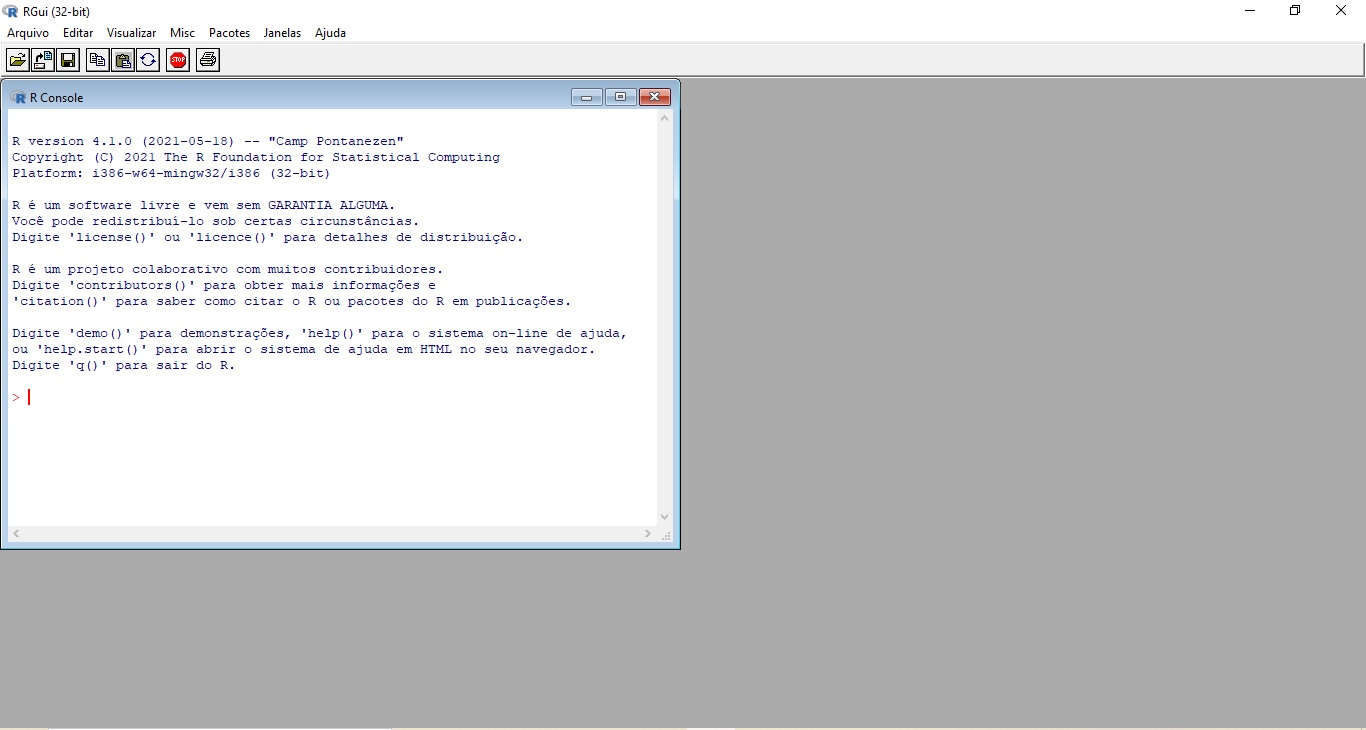
\includegraphics{C:/Users/eduar/OneDrive/Desktop/GitHub/disciplina_MFC/aula_00/auxiliar/R.png}

\hypertarget{opcional-r-studio}{%
\subsubsection{Opcional: R Studio}\label{opcional-r-studio}}

A interface do R pode parecer pouco amigável, principalmente para
usuários novos. Pensando nisso, a empresa RStudio desenvolveu uma IDE
(\emph{Integrated Development Environment}), o
\href{https://www.rstudio.com/}{RStudio}. O RStudio facilita a
utilização do R, ajudando o usuário a programar e fornecendo ferramentas
adicionais de compartilhamento e visualização. Para baixar o RStudio,
clique \href{https://www.rstudio.com/products/rstudio/download/}{aqui};
escolha a opção gratuíta (\emph{free}); e um arquivo .exe será baixado
em seu computador.

A instalação do RStudio requer que o R esteja instalado no seu
computador. Execute o arquivo .exe (e.g.~RStudio-1.4.1106.exe); escolha
as opções padrões. Fica a seu critério criar um atalho na sua área de
trabalho.

Se tudo deu certo, você será capaz de abrir o RStudio no seu computador.
A interface do RStudio será semelhante à seguinte:

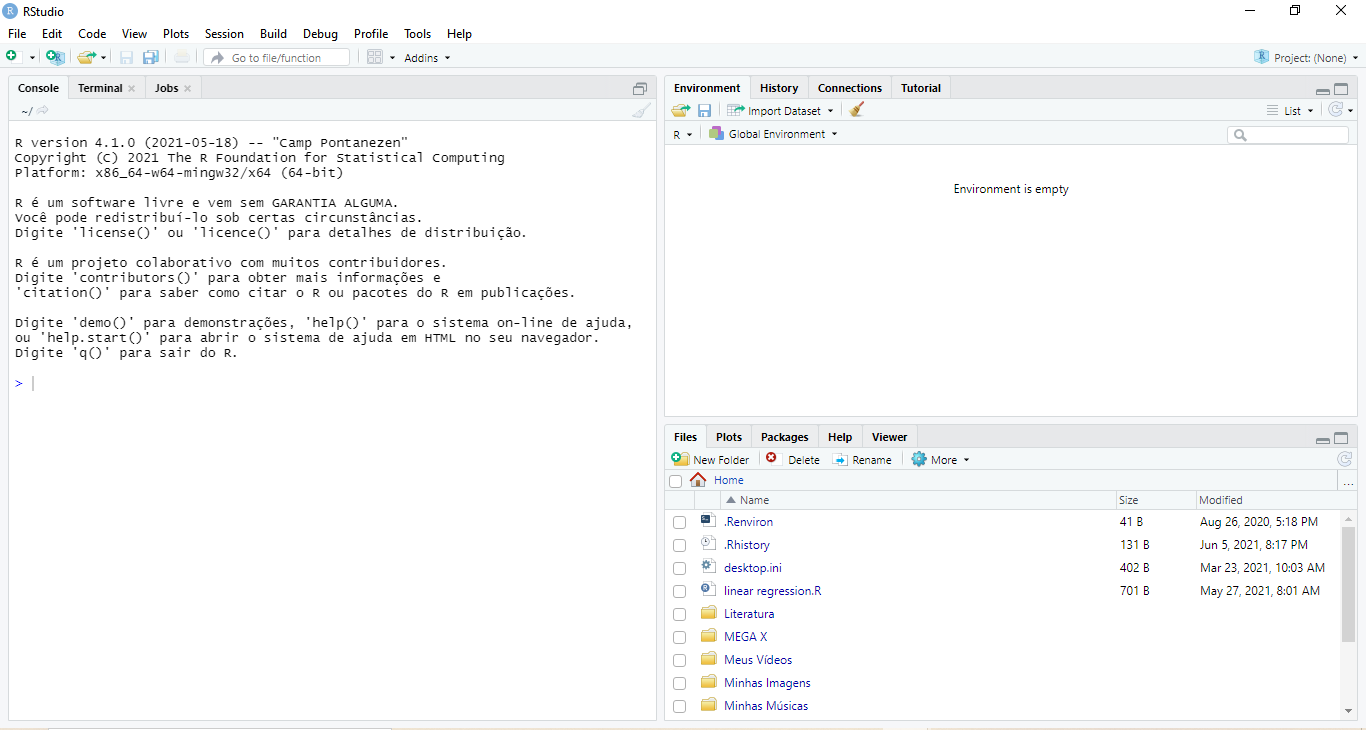
\includegraphics{C:/Users/eduar/OneDrive/Desktop/GitHub/disciplina_MFC/aula_00/auxiliar/RStudio.png}

\hypertarget{opcional-rstudio-cloud}{%
\subsubsection{Opcional: RStudio Cloud}\label{opcional-rstudio-cloud}}

Você pode estar com um computador com memória cheia, que talvez não
suporte o R ou o RStudio. Isto não será um impedimento para que você
acompanhe o minicurso. Existe uma opção \emph{online} do RStudio, o
\href{https://rstudio.cloud/}{RStudio Cloud}. Para ter acesso ao RStudio
Cloud, faça seu registro
\href{https://login.rstudio.cloud/register?redirect=\%2Foauth\%2Fauthorize\%3Fredirect_uri\%3Dhttps\%253A\%252F\%252Frstudio.cloud\%252Flogin\%26client_id\%3Drstudio-cloud\%26response_type\%3Dcode\%26show_auth\%3D0\%26show_login\%3D1\%26show_setup\%3D0\&setup=False}{aqui}.
Feito o registro, faça \emph{login} na sua conta. A primeira página será
a área dos seus projetos (\emph{Your Workspace}); clique em novo projeto
(\emph{New Project}) para carregar a interface do RStudio \emph{online}.
Se tudo deu certo, você terá acesso a uma página semelhante a essa:

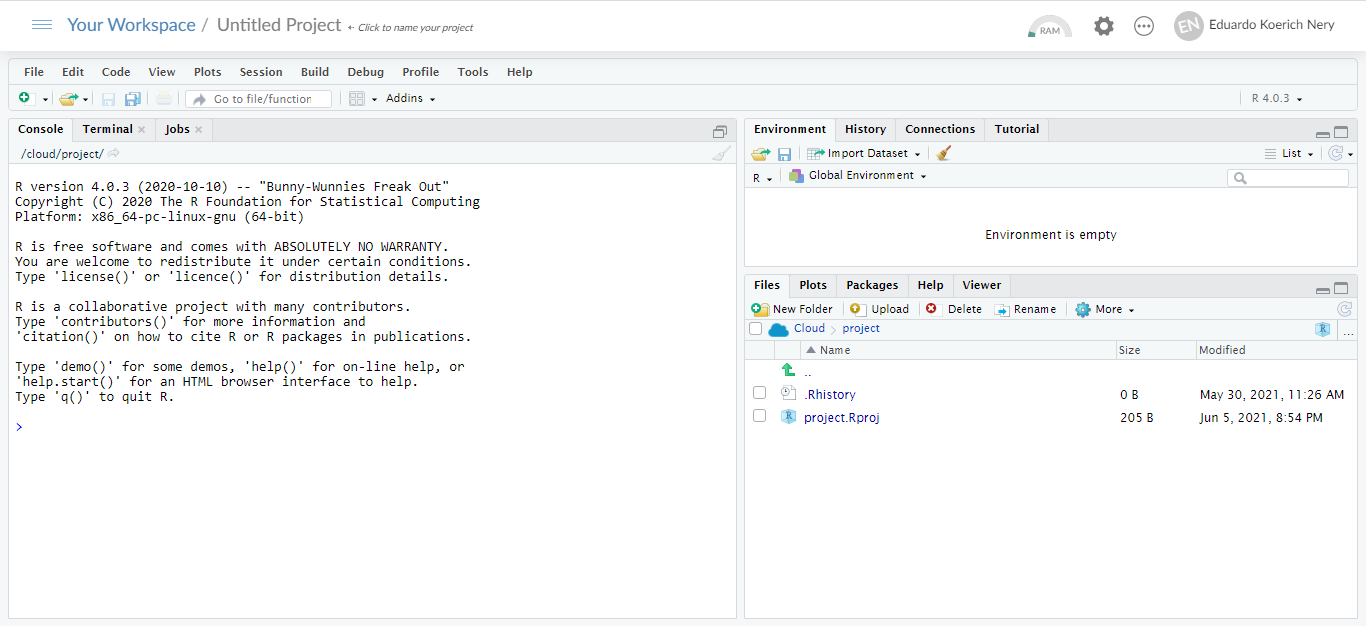
\includegraphics{C:/Users/eduar/OneDrive/Desktop/GitHub/disciplina_MFC/aula_00/auxiliar/RStudio_cloud.png}

\hypertarget{dificuldades}{%
\subsubsection{Dificuldades?}\label{dificuldades}}

Se ao longo desta aula você não conseguiu instalar/executar o R ou
acessar o RStudio Cloud, por favor, entre em contato comigo
(\href{mailto:eduardo.nery@ufabc.edu.br}{\nolinkurl{eduardo.nery@ufabc.edu.br}}).

\end{document}
